\section{}

\subsection{Useful Relations}\label{app:apx:useful}

%\subsubsection*{Bounding Absolute Value of $\FBCo$ and $\FBCt$ Integrands}
%First, we note that $\big|\real{Ze^{ib}}\big|\leq|Ze^{ib}|=|Z|$ holds for all $Z\in\C$ and
%$b\in\R$. Thus, we bound the absolute value of the integrand in \eqref{eq:apx:FBC1req1} for any 
%$\upxi,x\in\R^n$ and $b\in\R$ as
%\begin{align}\nonumber
%\big|\cos(\xidx+b)-\cos(b)\big| \ \leq \ \big|(e^{i\xidx}-1)e^{ib}\big| = 
%\big|e^{i\xidx}-1\big| 
%&= 
%2\big|\sin(\tfrac{\xidx}{2})\big| \\\label{eq:appApx:intgBnd1}
%&\leq 2\big|\tfrac{\xidx}{2}\big| = \big|\xidx\big| \ \ ,
%\end{align}
%which gives $|\cos(\xidx)-1|\leq|\xidx|$ for $b=0$.
%
%By then also noting $|\sin(0)-0|=0$ and $\tfrac{\d}{\d y}(\sin(y)-y)=\cos(y)-1$ for $y\in\R$, we
%can show that
%\begin{align*}
%|\sin(y)-y| = \left|\int_0^y\cos(z)-1\,\d z\right| \ \leq \ 
%\int_0^y|\cos(z)-1|\,\d z \ \leq \  \int_0^y|z|\,\d z = \tfrac{1}{2}|y|^2 \ \ .
%\end{align*}
%Combining these results, we bound the absolute value of the integrand in 
%\eqref{eq:apx:FBC2req1} 
%as
%\begin{align}\nonumber
%|\cos(\xidx+b)+\xidx\sin(b)-\cos(b)| \ &\leq \ |e^{i\xidx}-i\xidx-1| \\ \nonumber
%&= \sqrt{(\cos(\xidx)-1)^2 + (\sin(\xidx)-\xidx)^2} \\ \nonumber
%&\leq |\cos(\xidx)-1| + |\sin(\xidx)-\xidx| \\ \nonumber
%&= 2|\sin(\tfrac{\xidx}{2})|^2 + |\sin(\xidx)-\xidx| \\ \nonumber
%&\leq 2|\tfrac{\xidx}{2}|^2 + \tfrac{1}{2}|\xidx|^2 \\ \label{eq:appApx:intgBnd2}
%&= |\xidx|^2 \ \ .
%\end{align}
%
%\subsubsection*{Integrability of $\FBCo$ and $\FBCt$ Classes}
%We note here that the integrability of \eqref{eq:apx:FBC1req1} and \eqref{eq:apx:FBC2req1} are 
%given by using \eqref{eq:appApx:intgBnd1},\eqref{eq:apx:FBC1req2} and 
%\eqref{eq:appApx:intgBnd2},\eqref{eq:apx:FBC2req2} respectively, along with the definition of 
%$\abs{\upxi}_\Bc=\sup_{x\in\Bc}\abs{\xidx}$, as
%\begin{align*}
%\int_{\R^n} |e^{i\xidx}-1|\,G(\dxi) \ &\leq \ \int_{\R^n} |\xidx|\,G(\dxi) \ \leq \
%\int_{\R^n} \abs{\upxi}_\Bc\,G(\dxi) \ \leq \ \Cgo \\
%\int_{\R^n} |e^{i\xidx}-i\xidx-1|\,G(\dxi) \ &\leq \ \int_{\R^n} |\xidx|^2\,G(\dxi) \ \leq \
%\int_{\R^n} \abs{\upxi}_\Bc^2\,G(\dxi) \ \leq \ \Cgt \ \ .
%\end{align*}
%which is satisfied for all $x\in\Bc\subseteq B_0(\rho)$ since $\norm{x}_2\leq\rho$.

\subsubsection*{Reverse Triangle Inequality}

Let $\Fc$ be some function space with $f,g\in\Fc$. Let $\|\cdot\|$ be any norm
on $\Fc$. Then we have:
\begin{align*}
\|f\| = \|f - g + g\| \ &\leq \ 
\|f - g\| + \|g\| \\ 
\|g\| = \|g - f + f\| \ &\leq \ 
\|g - f\| + \|f\| = \|f-g\| + \|f\| \ \ ,
\end{align*}
due to the triangle inequality. Therefore, it holds that
\begin{equation}\label{eq:appApx:revTri}
\big|\,\|f\|-\|g\|\,\big| \ \leq \ \|f-g\| \ \ .
\end{equation}\\


\subsubsection*{Norm Difference for Functions with Different Coefficients}

Let $\Fc$ be some function space with $f,g\in\Fc$. Let $\|\cdot\|$ be any norm
on $\Fc$, and $a,b\in\R$. Then we have:
\begin{equation}\label{eq:appApx:normDiffCoef}
\|af-bg\| = \|a(f-g) - \Delta g\|
\leq
|a|\,\|f-g\| + |\Delta|\,\|g\|
\end{equation}
where $\Delta=b-a$, by using the triangle inequality.\\\\


\subsubsection*{Bounding Expected Variation of Sample Average Function from its Mean}

Let $\fb,\fb_1,\dots,\fb_N$ be drawn iid from a function space $\Fc$ and define the
sample average function $\fbbN=\frac{1}{N}\sum_{i=1}^N\fb_i$. With the $L_2(\Bc,\mu)$ norm (for
any valid measure $\mu$) denoted as $\normB{\cdot}$, we have
\begin{align}\nonumber
\E\normB{\fbbN - \E\fbbN}^2 \ &= \ \E\int_\Bc \left(\fbbN - \E\fbbN\right)^2\mu(\dx) \\ \nonumber
&\overset{(a)}{=} \ \int_\Bc \left(\E\left[\fbbN^{\,2}\right]
-2\,\E\left[\fbbN\right]\E\left[\fbbN\right]
+ \E\left[\fbbN\right]^2 \right)\mu(\dx) \\ \nonumber
&\overset{(b)}{=} \ \int_\Bc \left(\E\left[\fbbN^{\,2}\right] -
\E\left[\fbbN\right]^2 \right)\mu(\dx) \ 
= \int_\Bc \text{var}\!\left(\fbbN\right)\mu(\dx) \\ \nonumber
&\overset{(c)}{=} \ \int_\Bc \frac{1}{N}\,\text{var}(\fb)\,\mu(\dx) \ 
= \ \frac{1}{N} \int_\Bc \left(\E\left[\fb^2\right]-\E[\fb]^2\right)\mu(\dx) \\ 
\label{eq:appApx:varBnd}
&= \ \frac{1}{N}\left(\E\normB{\fb}^2-\normB{\E[\fb]}^2\right) \ 
\overset{(d)}{\leq} \ \frac{1}{N}\,\E\normB{\fb}^2 \ \ .
\end{align}
Here (a) is by using Fubini's theorem to bring the expectation inside the integral, the
linearity of expectation, and the outer expectation then being redundant for the last term, (b)
is from combining the middle and last terms, (c) is by the facts of variance of averaged iid
random variables (covariance terms are zero, while means and variances are equal), and (d) is
because the second term is nonpositive and therefore it can be dropped with inequality.\\\\


\subsubsection*{McDiarmid's Inequality}\label{sec:app:McDInq}

Let $\vb_1,\dots,\vb_d$, for any $d\in\N$, be independent random variables in the sets
$\Vc_1,\dots,\Vc_d$ and let the function $h:\Vc_1\times\dots\times\Vc_d\to\R$ satisfy for all
$i\in[d]$ and some positive scalars $k_1,\dots,k_d>0$, that
\begin{equation*}
|h(v_1,\dots,v_i,\dots,v_d)-h(v_1,\dots,\widetilde v_i,\dots,v_d)|\leq k_i
\end{equation*}
holds for all points $(v_1,\dots,v_i,\dots,v_d),(v_1,\dots,\widetilde v_i,\dots,v_d)\in
\Vc_1,\times\dots\times\Vc_d$ differing only at $v_i,\widetilde v_i\in\Vc_i$. Then, for all 
$t\geq0$, it holds that
\begin{equation}\label{eq:appApx:McDIneq}
\P\Big[\,h(\vb_1,\dots,\vb_d)-\E[h(\vb_1,\dots,\vb_d)]\,\geq t\,\Big]
\ \leq \ \exp\left(\frac{-2\,t^2}{\sum_{i=1}^dk_i^2}\right) \ \ .
\end{equation}

\newpage
\subsubsection*{Lemma on Approximating Functions of Convex Combinations}

The following lemma is credited to Maurey in \cite{pisier1981remarques}.

\begin{lemma}\label{lem:appApx:convComb}
%\begin{customlemma}{A.1}\label{lem:convComb}
If $\fch$ is in the closure of the convex hull of a bounded set of functions $\Fc$ in a Hilbert
space $\Hc$, such that $\norm{f}_{\Hc}\leq b$ holds for all $f\in\Fc$, then for every $N\geq1$,
there exists an $\fbN$ in the convex hull of $N$ points in $\Fc$ such that
\begin{equation*}
\norm{\fch-\fbN}_{\Hc}^2 \ \leq \ \frac{\bar{c}}{N}
\end{equation*}
holds for any $\bar{c} > b^2 - \norm{\fch\,}_{\Hc}^2 \ $.
%\end{customlemma}
\end{lemma}
\begin{proof}
Define $\fst$ as a finite but arbitrarily large convex combination of $m$ points
$\fst_i\in\Fc$, meaning it has the form $\fst = \sum_{i=1}^m\gamma_i\fst_i$ with $\gamma_i\geq0$, $\sum_{i=1}^m\gamma_i=1$, and such that
$\norm{\fch-\fst}_{\Hc}\leq\frac{\delta}{\sqrt{N}}$ for some $\delta>0$. Randomly sample
functions $\fb,\fb_1,\dots,\fb_N$ iid from the set $\{\fst_i,\dots,\fst_m\}$ according to
$\P[\fb=\fst_i]=\gamma_i$. Thus, we have $\E[\fbbN]=\E[\frac{1}{N}\sum_{i=1}^N\fb_i]=\E[\fb]
=\fst$, and then using \eqref{eq:appApx:varBnd} gives
$\E\norm{\fbbN-\fst}_{\Hc}^2=\frac{1}{N}(\E\norm{\fb}_{\Hc}^2 - \norm{\fst}_{\Hc}^2) \leq
\frac{1}{N}(b^2 - \norm{\fst}_{\Hc}^2)$. Since the expectation is bounded this way, there must
be a realization $\fbN$ that also satisfies this bound. Then by the triangle inequality, we have
$\norm{\fch-\fbN}_{\Hc} \leq \norm{\fch-\fst}_{\Hc} + \norm{\fbN-\fst}_{\Hc} =
\frac{1}{\sqrt{N}}(\delta + \sqrt{b^2 - \norm{\fst}_{\Hc}^2})$. And since $\fst$ can get
arbitrarily close to $\fch$ by letting $m\to\infty$, and thus $\delta\to0$ and
$\norm{\fst}_{\Hc}\to\norm{\fch\,}_{\Hc}$, this proves the result.
\end{proof}
In our setting, we use the $\normB{\cdot}$ norm for the $L_2(\Bc)$ space. We note that Theorem 1
of \cite{makovoz1996random} gives the same $O(\frac{1}{\sqrt{N}})$ result, but with a superior
constant. The proof there uses the same method as above, but breaks $\Fc$ into $N$ subsets of
diameter $\epsilon$, and then uses that to bound the variance terms. This gives the bound
constant in terms of an inverse covering number of $\Fc$ (denoted $\epsilon_N(\Fc)$), which goes
to zero as $N\to\infty$. However, this requires quantifying $\epsilon_N(\Fc)$, which may be
nontrivial.
%\newpage


%\section{Proof of Theorem~\ref{thm:apx:barron93}}\label{app:apx:barron93Proof}
%We closely follow the proof methods in \cite{barron1993universal}.
%Recalling that $g(x)=f(x)$, and thus $\widecheck{g}(x)=\fch(x)$, on $\Bc$, then taking the real 
%part of both sides of \eqref{eq:apx:FBC1req1} gives for all $x\in\Bc$ that
%\begin{align*}
%\real{\,\widecheck{g}(x)} \ = \ \real{\fch(x)} 
%=& \ \real{\int_{\R^n} (e^{i\xidx}-1)\,e^{i\phi(\upxi)}G(\dxi)} \\
%\fch(x) \ =& \ \int_{\R^n}\Big(\!\cos\big(\xidx + \phi(\upxi)\big) -
%\cos\big(\phi(\upxi)\big)\Big)\,G(\dxi) \\
%=&\ \int_{\Omega} h(x,\upxi)\,\Lambda(\dxi)
%\end{align*} 
%where $\Omega=\R^n\setminus\{0_n\}$ and equality is maintained because the integrand at 
%$\upxi=0_n$ is zero. Here, we defined
%\begin{align*}
%h(x,\upxi) &:= \frac{\Cgo}{\absB{\upxi}}\Big(\!\cos\big(\xidx + \phi(\upxi)\big)
%-\cos\big(\phi(\upxi)\big)\Big) \\[6pt]
%%\qquad\text{and}\qquad \\
%\Lambda(\dxi) &:= \frac{\absB{\upxi}}{\Cgo}\,G(\dxi)
%\end{align*}
%with $\Cgo$ as in \eqref{eq:apx:FBC1req2}, and so $\Lambda$ is a probability measure over 
%$\Omega$
%such that $\int_{\Omega}\Lambda(\dxi)=1$. Then by \eqref{eq:appApx:intgBnd1} and recalling the 
%definition of $\absB{\upxi}=\sup_{x\in\Bc}\abs{\xidx}$, it holds for all $x\in\Bc$ and 
%$\upxi\in\Omega$ that
%\begin{align*}
%|h(x,\upxi)| \ &\leq \ \frac{\Cgo}{\absB{\upxi}}\,|\xidx| \ \leq\ 
%\Cgo \ \leq\ C \ \ .
%\end{align*}
%With $\upxib,\upxib_1,\dots,\upxib_N\in\Omega$ sampled iid according to $\Lambda$, we have
%$\E[\frac{1}{N}\sum_{i=1}^Nh(x,\upxib_i)]=\fch(x)$. Thus, by \eqref{eq:appApx:varBnd} we have
%\begin{align*}
%\E\normB{\fch(x) -  \frac{1}{N}\sum_{i=1}^Nh(x,\upxib_i)}^2 \ \leq \ 
%\frac{1}{N}\,\E\normB{h(x,\upxib)}^2 \ \leq \ 
%\frac{1}{N} \int_\Bc C^2\,\muBdx = \frac{C^2}{N} \ \ .
%\end{align*}
%Since this goes to zero as $N\to\infty$, we have that for every $f\in\FBCo$, it holds over
%$x\in\Bc$ that $\fch\in\covcl\,\Hc_{C,\Bc}^{\cos(1)}\ $, where
%\newpage
%\begin{align*}
%\Hc_{C,\Bc}^{\cos(1)}\ :=\ \left\{\frac{\alpha}{\absB{\upxi}}\,\big(\cos(\xidx+b)
%- \cos(b)\big)\ \ \Big| \ \ \upxi\in\Omega , \ |\alpha|\leq C , \ b\in\R \right\}
%\end{align*}
%with closure in the sense of the $L_2(\Bc,\muB)$ norm.
%
%Next, for any $\upxi\in\Omega$ we set $y=\frac{1}{\absB{\upxi}}\xidx$, which gives
%$y\in\Yc\subseteq[-1,1]$ over $x\in\Bc$. Therefore, functions in $\Hc_{C,\Bc}^{\cos(1)}$ 
%correspond to smooth univariate functions of $y$ having the form
%\begin{align*}
%h(y) = \frac{\alpha}{\absB{\upxi}}\,\big(\cos(\absB{\upxi}y+b) - \cos(b)\big)
%\end{align*}
%for any $\upxi\in\Omega$, $|\alpha|\leq C$, and $b\in\R$, and thus having derivative
%$$
%h'(y) = -\alpha\sin(\absB{\upxi}y+b)\ \ .
%%\qquad\text{and}\qquad
%%h''(y)=-\alpha\absB{\upxi}\cos(\absB{\upxi}y+b) \ \ .
%$$
%These $h(y)$ functions are uniformly continuous and bounded on $y\in[-1,1]$ with $h(0)=0$ and
%$|h(y)|\leq C$, and so they can be uniformly approximated on this interval by piecewise constant
%functions. Setting a uniform partition of $[0,1]$ for any positive integer $P$ as
%$\Delta:=\frac{1}{P} < 2\Delta < \cdots < (P-1)\Delta < P\Delta=1$, we define
%\begin{align*}
%h_{2P}(y) := \sum_{\dscr\in\{-1,1\}}\!&\left(
%h(0)\,\step(\dscr y)
%%\right. \\
%%&+ \ 
%%\left.
%+ \sum_{k=1}^{P-1}\big(h(\dscr k\Delta) + 
%h(\dscr(k-1)\Delta)\big)\,\step(\dscr y-k\Delta)\right) \ \ ,
%\end{align*}
%recalling that $\step(y)=\Ind[y>0]$ is the step activation function. This definition means
%$h_{2P}$ is a continuous, length $2P$ sequence of constant lines on $y\in[-1,1]$ between each
%pair of points $\big\{h(\dscr(k-1)\Delta),h(\dscr k\Delta)\big\}$, over $k\in[P]$ and 
%$\dscr\in\{-1,1\}$.
%
%Thus, as $P\to\infty$ (and $\Delta\to0$) we get $h_{2P}\to h$ uniformly on $y\in[-1,1]$, and the
%absolute values of the coefficients are
%\begin{align*}
%|h(0)|=0 
%\quad\text{and}\quad
%|h(\dscr k\Delta)-h(\dscr(k-1)\Delta)| \ \ .
%\end{align*}
%By definition, the sum of the absolute values of the coefficients is then bounded by the total
%variation of $h'(y)$ over $y\in[-1,1]$. And since
%$|h'(y)|=|\alpha||-\sin(\absB{\upxi}y+b)|\leq C$, we have for any $P\geq1$ that
%\begin{align*}
%\sum_{\dscr\in\{-1,1\}}\!&\left(\abs{h(0)} + 
%\sum_{i=1}^{P-1}\abs{h(\dscr k\Delta)+h(\dscr(k-1)\Delta)}
%\right)
%\leq\  \int_{-1}^1|h'(y)|\,\d y \ \leq\ 2C \ \ .
%\end{align*}
%This proves that for every $f\in\FBCo$, it holds over $x\in\Bc$ that $\fch(x)\in
%\covcl\,\Hc_{C,\Bc}^\Sc$, where
%\begin{align*}
%\Hc_{C,\Bc}^\Sc\ :=\ 
%\big\{\alpha\,\step(\xidx+b) \ \ \big| \ \ |\alpha|\leq2C , \absB{\upxi}=1 , |b|\leq1\big\}
%\end{align*}
%with closure in the supremum norm over $x\in\Bc$, and thus also in the sense of the 
%$L_2(\Bc,\muB)$ norm.
%Recalling that we had defined $y=\frac{1}{\absB{\upxi}}\xidx$, which gave 
%$y\in\Yc\subseteq[-1,1]$ 
%for any $\upxi\in\Omega$, then $\xidx\in\Wc\subseteq[-\absB{\upxi},\absB{\upxi}]$ and thus why 
%$\absB{\upxi}=1$ 
%is specified in the definition of $\Hc_{C,\Bc}^\Sc$.
%
%To bound the $L_2(\Bc,\muB)$ norm for all functions in this set, note that the largest norms
%belong to the functions that correspond to $h(y)=(\pm2C)\step(\pm y+1)$, which over 
%$y\in[-1,1]$ 
%are equivalent to $(\pm2C)$. Thus, for all $h\in\Hc_{C,\Bc}^R$ we have
%$$
%\normB{h}^2 = \int_\Bc (\alpha\,\step(\xidx+b))^2\,\muBdx \ \leq \ 
%(\pm2C)^2\int_{-1}^1 1^2\,\mupmo(\d y) = (2C)^2 \ \ ,
%$$
%where $\mupmo(\d y)=\frac{1}{2}\d y$ is the uniform probability measure over $y\in[-1,1]$ such 
%that $\int_{-1}^1\mupmo(\d y)=\int_{-1}^1\frac{1}{2}\d y=1$.
%
%Using Lemma~\ref{lem:appApx:convComb} with $\bar{c}=\bs^2=(2C)^2$ (which is justified, since we
%can only have $\|\fch\,\|_\Bc^2=0$ if $\fch(x)=0$ for all $x\in\Bc$) then allows us to conclude
%that there must exist $\fhN$ in the convex hull of $N$ points in $\Hc_{C,\Bc}^\Sc$ satisfying
%$
%\|\fch-\fhN\|_\Bc \ \leq \ 2C\big(N^{-\frac{1}{2}}\big) \ 
%$.
%
%This means the approximation has the form
%$
%\fhN(x) = \sum_{i=1}^N u_i\,\alpha_i\step(\widx+b_i)
%$
%such that $\sum_{i=1}^Nu_i=1$ with $u_1,\dots,u_N\geq0$. Therefore, we can bound
%the coefficient size as
%$
%\sum_{i=1}^N|\theta_i| = \sum_{i=1}^Nu_i|\alpha_i| \ \leq \ \sum_{i=1}^Nu_i(2C)
%= 2C\,\sum_{i=1}^Nu_i = 2C $ for any $N\in\N$.
%\vphantom{a}\hfill$\blacksquare$
%\newpage
%
%\section{Proof of Theorem~\ref{thm:apx:brei93}}\label{app:apx:brei93Proof}
%We closely follow the proof methods in \cite{barron1993universal} and \cite{breiman1993hinging}.
%Recalling that $g(x)=f(x)$, and thus $\widecheck{g}(x)=\fch(x)$, on $\Bc$, then taking the real 
%part of both sides of \eqref{eq:apx:FBC2req1} gives for all $x\in\Bc$ that
%\begin{align*}
%\real{\,\widecheck{g}(x)} \ = \ \real{\fch(x)} 
%%\ =& \ \real{\int_{\R^n} (e^{i\xidx}-i\xidx-1)\,\Gw(\dxi)} \\
%=& \ \real{\int_{\R^n} (e^{i\xidx}-i\xidx-1)\,e^{i\phi(\upxi)}G(\dxi)} \\
%\fch(x) \ =& \ \int_{\R^n}\Big(\!\cos\big(\xidx + \phi(\upxi)\big) + 
%\xidx\,\sin\big(\phi(\upxi)\big)-
%\cos\big(\phi(\upxi)\big)\Big)\,G(\dxi) \\
%=&\ \int_{\Omega} h(x,\upxi)\,\Lambda(\dxi)
%\end{align*} 
%where $\Omega=\R^n\setminus\{0_n\}$ and equality is maintained because the integrand at 
%$\upxi=0_n$
%is zero. Here, we defined
%\begin{align*}
%h(x,\upxi) &:= \frac{\Cgt}{\absB{\upxi}^2}\Big(\!\cos\big(\xidx + \phi(\upxi)\big) + 
%\xidx\,\sin\big(\phi(\upxi)\big)-\cos\big(\phi(\upxi)\big)\Big) \\[6pt]
%%\qquad\text{and}\qquad \\
%\Lambda(\dxi) &:= \frac{\absB{\upxi}^2}{\Cgt}\,G(\dxi)
%\end{align*}
%with $\Cgt$ as in \eqref{eq:apx:FBC2req2}, and so $\Lambda$ is a probability measure over 
%$\Omega$
%such that $\int_{\Omega}\Lambda(\dxi)=1$. Then by \eqref{eq:appApx:intgBnd2} and recalling the 
%definition of $\absB{\upxi}=\sup_{x\in\Bc}\abs{\xidx}$, it holds for all $x\in\Bc$ and 
%$\upxi\in\Omega$ 
%that
%\begin{align*}
%|h(x,\upxi)| \ &\leq \ \frac{\Cgt}{\absB{\upxi}^2}\,|\xidx|^2 \ \leq\ 
%\Cgt \ \leq\ C \ \ .
%\end{align*}
%With $\upxib,\upxib_1,\dots,\upxib_N\in\Omega$ sampled iid according to $\Lambda$, we have
%$\E[\frac{1}{N}\sum_{i=1}^Nh(x,\upxib_i)]=\fch(x)$. Thus, by \eqref{eq:appApx:varBnd} we have
%\begin{align*}
%\E\normB{\fch(x) -  \frac{1}{N}\sum_{i=1}^Nh(x,\upxib_i)}^2 \ \leq \ 
%\frac{1}{N}\,\E\normB{h(x,\upxib)}^2 \ \leq \ 
%\frac{1}{N} \int_\Bc C^2\,\muBdx = \frac{C^2}{N} \ \ .
%\end{align*}
%Since this goes to zero as $N\to\infty$, we have that for every $f\in\FBCt$, it holds over
%$x\in\Bc$ that $\fch\in\covcl\,\Hc_{C,\Bc}^{\cos(2)}\ $, where
%\newpage
%\begin{align*}
%\Hc_{C,\Bc}^{\cos(2)}\ :=\ \left\{\frac{\alpha}{\absB{\upxi}^2}\,\big(\cos(\xidx+b) + \xidx\,
%\sin(b)- \cos(b)\big)\ \ \Big| \ \ \upxi\in\Omega , \ |\alpha|\leq C , \ b\in\R \right\}
%\end{align*}
%with closure in the sense of the $L_2(\Bc,\muB)$ norm.
%
%Next, for any $\upxi\in\Omega$ we set $y=\frac{1}{\absB{\upxi}}\xidx$, which gives
%$y\in\Yc\subseteq[-1,1]$ over $x\in\Bc$. Therefore, functions in $\Hc_{C,\Bc}^{\cos(2)}$ 
%correspond to smooth univariate functions of $y$ having the form
%\begin{align*}
%h(y) = \frac{\alpha}{\absB{\upxi}^2}\,\big(\cos(\absB{\upxi}y+b) + \absB{\upxi}y\,\sin(b)- 
%\cos(b)\big)
%\end{align*}
%for any $\upxi\in\Omega$, $|\alpha|\leq C$, and $b\in\R$, and thus having derivatives
%$$
%h'(y) = \frac{\alpha}{\absB{\upxi}}\,\big(-\sin(\absB{\upxi}y+b) + \sin(b)\big)
%\qquad\text{and}\qquad
%h''(y)=-\alpha\cos(\absB{\upxi}y+b) \ \ .
%$$
%These $h(y)$ functions are uniformly continuous and bounded on $y\in[-1,1]$ with $h(0)=0$ and
%$|h(y)|\leq C$, and so they can be uniformly approximated on this interval by piecewise linear
%functions. Setting a uniform partition of $[0,1]$ for any positive integer $P$ as
%$\Delta:=\frac{1}{P} < 2\Delta < \cdots < (P-1)\Delta < P\Delta=1$, we define
%\begin{align*}
%h_{2P}(y) := \sum_{\dscr\in\{-1,1\}}\!&\left(
%\frac{h(\dscr\Delta)-h(0)}{\Delta}\,\relu(\dscr y)\right. \\
%&+ \ 
%\left.\sum_{k=1}^{P-1}\frac{h(\dscr(k+1)\Delta)-2h(\dscr k\Delta) + 
%h(\dscr(k-1)\Delta)}{\Delta}\,\relu(\dscr y-k\Delta)\right) \ \ ,
%\end{align*}
%recalling that $\relu(y)=\max\{0,y\}$ is the ReLU activation function. This definition means
%$h_{2P}$ is a continuous, length $2P$ sequence of secant lines on $y\in[-1,1]$ between each pair
%of points $\big\{h(\dscr(k-1)\Delta),h(\dscr k\Delta)\big\}$, over $k\in[P]$ and 
%$\dscr\in\{-1,1\}$.
%
%Thus, as $P\to\infty$ (and $\Delta\to0$) we get $h_{2P}\to h$ uniformly on $y\in[-1,1]$, and the
%absolute values of the coefficients go to
%\begin{align*}
%%\label{eq:reluCoeffs}
%\abs{\frac{h(\dscr\Delta)-h(0)}{\Delta}} \ &\to \ |h'(0)|=0 \\
%%\quad\text{and}\quad
%\abs{\frac{h(\dscr(k+1)\Delta)-2h(\dscr k\Delta)+h(\dscr(k-1)\Delta)}{\Delta}} \ &\to \ 
%|h'(\dscr k\Delta)-h'(\dscr(k-1)\Delta)| \ \ .
%\end{align*}
%By definition, the sum of the absolute values of the coefficients is then bounded by the total
%variation of $h''(y)$ over $y\in[-1,1]$. And since
%$|h''(y)|=|\alpha||-\cos(\absB{\upxi}y+b)|\leq C$, we have for any $P\geq1$ that
%\begin{align*}
%\sum_{\dscr\in\{-1,1\}}\!&\left(\abs{\frac{h(\dscr\Delta)-h(0)}{\Delta}} + 
%\sum_{i=1}^{P-1}\abs{\frac{h(\dscr(k+1)\Delta)-2h(\dscr 
%k\Delta)+h(\dscr(k-1)\Delta)}{\Delta}}
%\right) \\
%&\leq\  \int_{-1}^1|h''(y)|\,\d y \ \leq\ 2C \ \ .
%\end{align*}
%%holds .\\\\
%This proves that for every $f\in\FBCt$, it holds over $x\in\Bc$ that $\fch(x)\in
%\covcl\,\Hc_{C,\Bc}^\Rc$, where
%\begin{align*}
%\Hc_{C,\Bc}^\Rc\ :=\ 
%\big\{\alpha\,\relu(\xidx+b) \ \ \big| \ \ |\alpha|\leq2C , \absB{\upxi}=1 , |b|\leq1\big\}
%\end{align*}
%with closure in the supremum norm over $x\in\Bc$, and thus also in the sense of the 
%$L_2(\Bc,\muB)$ norm.
%Recalling that we had defined $y=\frac{1}{\absB{\upxi}}\xidx$, which gave 
%$y\in\Yc\subseteq[-1,1]$ 
%for any $\upxi\in\Omega$, then $\xidx\in\Wc\subseteq[-\absB{\upxi},\absB{\upxi}]$ and thus why 
%$\absB{\upxi}=1$ 
%is specified in the definition of $\Hc_{C,\Bc}^\Rc$.
%
%To bound the $L_2(\Bc,\muB)$ norm for all functions in this set, note that the largest norms
%belong to the functions that correspond to $h(y)=(\pm2C)\relu(\pm y+1)$, which over 
%$y\in[-1,1]$ 
%are equivalent to $(\pm2C)(\pm y+1)$. Thus, for all $h\in\Hc_{C,\Bc}^R$ we have
%$$
%\normB{h}^2 = \int_\Bc (\alpha\,\relu(\xidx+b))^2\,\muBdx \ \leq \ 
%(\pm2C)^2\int_{-1}^1 (\pm y+1)^2\,\mupmo(\d y) = \tfrac{4}{3}(2C)^2 \ \ ,
%$$
%where $\mupmo(\d y)=\frac{1}{2}\d y$ is the uniform probability measure over $y\in[-1,1]$ such 
%that $\int_{-1}^1\mupmo(\d y)=\int_{-1}^1\frac{1}{2}\d y=1$.
%
%Using Lemma~\ref{lem:appApx:convComb} with $\bar{c}=\bs^2=\frac{4}{3}(2C)^2$ (which is 
%justified, since we can only have $\|\fch\,\|_\Bc^2=0$ if $\fch(x)=0$ for all $x\in\Bc$) then 
%allows us to conclude that there must exist $\fhN$ in the convex hull of $N$ points in 
%$\Hc_{C,\Bc}^\Rc$ satisfying
%$
%\|\fch-\fhN\|_\Bc \ \leq \ \sqrt{\frac{16}{3}}C\,\big(N^{-\frac{1}{2}}\big) \ 
%$.
%
%This means the approximation has the form
%$
%\fhN(x) = \sum_{i=1}^N u_i\,\alpha_i\relu(\widx+b_i)
%$
%such that $\sum_{i=1}^Nu_i=1$ with $u_1,\dots,u_N\geq0$. Therefore, we can bound
%the coefficient size as
%$
%\sum_{i=1}^N|\theta_i| = \sum_{i=1}^Nu_i|\alpha_i| \ \leq \ \sum_{i=1}^Nu_i(2C)
%= 2C\,\sum_{i=1}^Nu_i = 2C \ .
%$
%\vphantom{a}\hfill$\blacksquare$


\newpage
\section{Proof of Theorem~\ref{thm:apx:moll}}\label{app:apx:mollProof}
First, we observe that \eqref{eq:apx:baseIntRepLam} is equivalently
\begin{align}\nonumber
\fhN(x) \ = \ \sum_{i=1}^{N} \theta_i\,\sigma(\pariX)\,
\int_\Upsilonl \deltalno(\upgamma-\upgamma_i)\,\d\upgamma \ = \ 
\sum_{i=1}^{N} \theta_i\,\int_\Upsilonl \deltalno(\upgamma-\upgamma_i)\,\sigma(\pariX)\,
\d\upgamma \ ,
\end{align}
since $\int_\Upsilonl \deltalno(\upgamma-\upgamma_i)\,\d\upgamma=1$ holds for all $\lambda>0$, 
$n\geq1$, and $\upgamma_i\in\Upsilon$, and $\sigma(\pariX)$ is a constant with respect to
$\d\upgamma$.

Then we define the sets $\Upsilonil$ as the supports of each $\deltalno(\upgamma-\upgamma_i)$,
which is the open cube $(-\frac{1}{\lambda},\frac{1}{\lambda})^{n+1}$ centered at the 
corresponding $\upgamma_i\in\Upsilon$, and note that these are always contained within the
$\lambda$-expanded $\Upsilonl$. Therefore, for any $x\in\Bc$ we have
\begin{align}\nonumber
\big|\fhN(x) - \fhlN(x)\big| \ &=  \ 
%&\ \ \ \abs{ \, \sum_{i=1}^{N} \theta_i\,\int_\Upsilonl\deltalno(\upgamma-\upgamma_i)
%\,\sigma(\pariX)\,\d\upgamma \ - 
%\sum_{i=1}^{N} \theta_i\,\int_\Upsilonl \deltalno(\upgamma-\upgamma_i)\,\sigma(\upgamma^\top 
%z)\,\d\upgamma
% \, } \\ \nonumber
\left| \, \sum_{i=1}^{N} \theta_i\,\int_\Upsilonl\deltalno(\upgamma-\upgamma_i)
\,\Big(\sigma(\pariX) - \sigma(\parX)\Big)\,\d\upgamma \, \right| 
\\\nonumber
&\overset{(a)}{\leq}\ \sum_{i=1}^{N} \, |\theta_i| \, \left| 
\int_\Upsilonl\deltalno(\upgamma-\upgamma_i)
\,\Big(\sigma(\pariX) - \sigma(\parX)\Big)\,\d\upgamma \, \right| 
\\\nonumber
&\overset{(b)}{\leq}\ \sum_{i=1}^{N} \, |\theta_i| \, 
\int_\Upsilonl\deltalno(\upgamma-\upgamma_i)
\,\left|\sigma(\pariX) - \sigma(\parX)\right|\,\d\upgamma \\\nonumber
&\overset{(c)}{\leq}\ \sum_{i=1}^{N} |\theta_i| \int_\Upsilonl\deltalno(\upgamma-\upgamma_i)
\sup_{\phi\in\Upsilonil}\left|\sigma(\pariX) - \sigma(\phi^\top X)\right|\d\upgamma
\\\nonumber
&\overset{(d)}{=}\ \sum_{i=1}^{N} |\theta_i| \sup_{\phi\in\Upsilonil}\left|\sigma(\pariX) -
\sigma(\phi^\top X)\right| \int_\Upsilonl\deltalno(\upgamma-\upgamma_i)\d\upgamma \\ \nonumber
&\overset{(e)}{=}\ \Sc_N \sup_{\phi\in\Upsilonil}\left|\sigma(\pariX) -
\sigma(\phi^\top X)\right|
\ \ .
\end{align}
Here (a) is by the triangle inequality, (b) is because $\left|\int
f(x)\,\d x\right|\leq\int|f(x)|\,\d x$ and $\deltalno$ is positive, (c) is because the
integrand is only nonzero on $\upgamma\in\Upsilonil$ by the support of $\deltalno$, (d) is 
because the sup is a constant and can thus be pulled out of the integral, and (e) is by the 
definition of the mollified delta such that 
$\int_\Upsilonl\deltalno(\upgamma-\upgamma_i)\d\upgamma=1$ for all $i\in[N]$ and the (assumed 
known) bound $\sum_{i=1}^N|\theta_i|\leq \Sc_N$.

If $\sigma$ satisfies the overall boundedness assumption with constant $\Dsig$, then we have
\begin{align}\nonumber
\big|\fhN(x) - \fhlN(x)\big| \ 
= \ \Sc_N \, \Dsig
\end{align}
and thus
\begin{align*}
\normB{\fhN(x)-\fhlN(x)} \ &\leq \ 
\sqrt{\int_\Bc \abs{\Sc_N \,\Dsig}^2\,\muBdx} \ = \ \Sc_N \,\Dsig
\end{align*}
where $\Sc_N$ and $\Dsig$ are positive constants.

Otherwise, $\sigma$ satisfies the Lipschitz assumption with constant $\Lsig$ and so we have
\begin{align}\nonumber
\big|\fhN(x) - \fhlN(x)\big| \ 
&\leq \ \Sc_N \, \Lsig
\sup_{\phi\in\Upsilonil}\left|(\upgamma_i -\phi)^\top X\, \right| \\ 
\label{eq:appApx:absDifffNflN}
&\overset{(f)}{\leq} \ \Sc_N \, \frac{\Lsig\,\sqrt{n+1}}{\lambda}\,\|X\|_2
\end{align}
where (f) uses the Cauchy-Schwarz inequality, combined with the fact that
$\|\upgamma_i-\phi\|_2\leq\frac{\sqrt{n+1}}{\lambda}$ for all $\phi\in\Upsilonil$ at any 
$\upgamma_i\in\Upsilonl$. And thus
\begin{align*}
\normB{\fhN(x)-\fhlN(x)} \ &\leq \
\sqrt{\int_\Bc \abs{\Sc_N \,\frac{\Lsig\,\sqrt{n+1}}{\lambda}\,\|X\|_2}^2\,\muBdx} \ = \ 
\Sc_N\ \frac{\Lsig\,\sqrt{n+1}}{\lambda}\ \EB
\end{align*}
where $\Sc_N$, $\Lsig$, $\sqrt{n+1}$, and $\lambda$ are all positive constants.
\vphantom{a}\hfill$\blacksquare$

\newpage


\section{Proof of Lemma~\ref{lem:apx:exp}}\label{app:apx:exp}
The mollified approximation $\fhlN$ has the integral approximation \eqref{eq:apx:mollApx}, which
can be equivalently written as
%\begin{equation}\label{eq:apx:mollApx}
$$
\fhlN(x) := \int_\Upsilonl \gl(\upgamma_i)\ \sigma(\upgamma^\top
z)\,\d\upgamma
% \hspace{40pt} \forall x\in\Bc \ \ ,
$$
where coefficient function $\gl$ is defined in \eqref{eq:apx:gLam}. Then with $\Pl$ being the
known nonzero density over $\Upsilonl$ used for sampling the parameters, we can equivalently 
write this as
\begin{equation}\label{eq:apx:intRep2}
\fhlN(x) = \int_\Upsilonl \frac{\gl(\upgamma)}{\Pl(\upgamma)}\,\sigma(\upgamma^\top z)
\,\Pl(\upgamma)\d\upgamma
= \Exp_{\upgammab\sim\Pl}\limits
\left[\frac{\gl(\upgammab)}{\Pl(\upgammab)}\,\sigma(\upgammab^\top z)\right]
%\hspace{40pt} \forall x\in\Bc
\ \ .
\end{equation}
For any sampled parametervalues $\upgammab_1,\dots,\upgammab_R$ from $\Upsilonl$, let us denote
$\ftr^*$ as the random approximation that has coefficient values $\vartheta^*\in\R^R$ of
\begin{equation}\label{eq:appApx:cjOpt}
\vartheta_j^*\ =\ \frac{\gl(\upgammab_j)}{\Pl(\upgammab_j)\,R} \ 
=\ \frac{\sum_{i=1}^N\theta_i\,\deltalno(\upgammab_j-\upgamma_i)}{\Pl(\upgammab_j)\,R}
\hspace{40pt}\forall j\in[R] \ \ .
\end{equation}
Let us denote $\d\Pl(\upgamma_j):=\Pl(\upgamma_j)\,\d\upgamma_j$ for all $j\in[R]$, so that in 
the below integrals $\upgamma,\upgamma_1,\dots,\upgamma_R$ all represent separate variables of
integration. Then with the iid assumption on all $\upgammab_j\sim\Pl$, for this $\ftr^*$ we have
\begin{align*}
\Exp_{\upgammab_j\sim\Pl}\limits&\left[\ftr^*(x\,;\upgammab_1,\dots,\upgammab_R)\right]\  = \ 
\Exp_{\upgammab_j\sim\Pl}\limits\left[\sum_{j=1}^{R}\vartheta_j^*\,\sigma(\upgammab_j^\top 
z)\right] \\
&= \ \int_\Upsilonl\cdots\int_\Upsilonl\ \sum_{j=1}^R\frac{\gl(\upgamma_j)}{\Pl(\upgamma_j)\,R}\,
\sigma(\upgamma_j^\top z)\ \d\Pl(\upgamma_1)\,\cdots\,\d\Pl(\upgamma_R) \\
&\overset{(a)}{=}\ \int_\Upsilonl\cdots\int_\Upsilonl \frac{\gl(\upgamma_1)}{\Pl(\upgamma_1)\,R}\,
\sigma(\upgamma_1^\top z)\,\d\Pl(\upgamma_1)\,\cdots\,\d\Pl(\upgamma_R) \ + \ \cdots \\
& \hspace{100pt} + \ \int_\Upsilonl\cdots\int_\Upsilonl \frac{\gl(\upgamma_R)}{\Pl(\upgamma_R)\,R}\,
\sigma(\upgamma_R^\top z)\,\d\Pl(\upgamma_1)\,\cdots\,\d\Pl(\upgamma_R) \\
&\overset{(b)}{=}\ \int_\Upsilonl\frac{\gl(\upgamma_1)}{\Pl(\upgamma_1)\,R}\,
\sigma(\upgamma_1^\top z)\,\d\Pl(\upgamma_1)\  \big(1^{R-1}) \ + \ \cdots \\
& \hspace{150pt} + \int_\Upsilonl\frac{\gl(\upgamma_R)}{\Pl(\upgamma_R)\,R}\,
\sigma(\upgamma_R^\top z)\,\d\Pl(\upgamma_R)\ \big(1^{R-1}) \\
&\overset{(c)}{=}\ R \left(\frac{1}{R}\int_\Upsilonl \frac{\gl(\upgamma)}{\Pl(\upgamma)}\,
\sigma(\upgamma^\top z)\, \d\Pl(\upgamma) \right) \ \ 
\overset{(d)}{=} \ \fhlN(x) 
%\hspace{40pt} \forall x\in\Bc 
\ \ .
\end{align*}
Here, (a) is by the linearity of integration, (b) is each $\upgamma_j$ only belongs to the
$\d\Pl(\upgamma_j)$ integral, while the remaining $R-1$ integrals in each term are
$\int_{\Upsilonl}\d\Pl(\upgamma_j)=1$, (c) is because there are $R$ copies of the same integral, and
(d) is \eqref{eq:apx:intRep2}.
\vphantom{a}\hfill$\blacksquare$ 


%\section{Proof of Lemma~\ref{lem:apx:hprops}}\label{app:apx:hpropsProof}
%Since $\fhR$ is assumed to satisfy Lemma~\ref{lem:apx:exp}, then by \eqref{eq:appApx:cjOpt}
%it holds for all $j\in[R]$ that
%\begin{equation}\label{eq:appApx:cMax}
%|\vartheta_j|\ \leq\ \left|\frac{\gl(\upgammab_j)}{\Pl(\upgammab_j)\,R}\right| \ \leq\
%\frac{\Cgl}{\pmin\,R} \ \ ,
%\end{equation}
%where $\Cgl$ is defined in \eqref{eq:apx:Cgl} and $\pmin:=\min\{\Pl(\upgamma)\ |\ 
%\upgamma\in\Upsilonl\}$.
%
%From the definition of $h_\Bc$ in \eqref{eq:apx:hB}, and for all points differing only at
%\mbox{coordinate $j$} as 
%$(\upgamma_1,\dots,\upgamma_j,\dots,\upgamma_R),(\upgamma_1,\dots,\upgammaw_j,\dots,
%\upgamma_R)\in\Upsilon^R_\lambda$, we have for all $j\in[R]$ that
%\begin{align}\nonumber
%\big|h_\Bc(&\upgamma_1,\dots,\upgamma_j,\dots,\upgamma_R)- 
%h_\Bc(\upgamma_1,\dots,\upgammaw_j,\dots,\upgamma_R)\big| \\ \nonumber
%&=\ \Big|\,\normB{\fhlN(x) - \fhR(x\,;\upgamma_1,\dots,\upgamma_j,\dots,\upgamma_R)} 
%- \normB{\fhlN(x) - \fhR(x\,;\upgamma_1,\dots,\upgammaw_j,\dots,\upgamma_R)}\,\Big|\\ 
%\nonumber
%&\overset{(a)}{\leq}\ \big\|\fhlN(x) - \fhR(x\,;\upgamma_1,\dots,\upgamma_j,\dots,\upgamma_R) 
%- \fhlN(x) + \fhR(x\,;\upgamma_1,\dots,\upgammaw_j,\dots,\upgamma_R) \big\|_B 
%\\\nonumber
%&\overset{(b)}{=}\ \normB{\frac{\gl(\upgammaw_j)}{\Pl(\upgammaw_j)\,R}\,
%\sigma(\upgammaw_j^\top X) - \frac{\gl(\upgamma_j)}{\Pl(\upgamma_j)\,R}\,
%\sigma(\parjX) } \\[5pt] \nonumber
%&\overset{(c)}{\leq}\ \abs{\frac{\gl(\upgammaw_j)}{\Pl(\upgammaw_j)\,R}}
%\normB{\sigma(\upgammaw_j^\top X) - \sigma(\parjX)} + 
%\bigg|\frac{\gl(\upgamma_j)}{\Pl(\upgamma_j)\,R}-\frac{\gl(\upgammaw_j)}{\Pl(\upgammaw_j)\,R}\bigg|
%\normB{\sigma(\parjX)} \\[5pt] \nonumber
%&\overset{(d)}{\leq}\ \frac{\Cgl}{\pmin\,R} \bigg(\normB{\sigmach(\upgammaw_j^\top X) -
%\sigmach(\parjX)} + 2 \normB{\sigmach(\parjX)} + 2\abs{\sigma(0)} \bigg) 
%\end{align}
%Here, (a) is by the reverse triangle inequality
%\eqref{eq:appApx:revTri}, (b) is by the definition of $\fhR$ such that only $\vartheta_j$ 
%differs at
%$\upgamma_j\neq\upgammaw_j$, (c) is by the inequality \eqref{eq:appApx:normDiffCoef}, (d) is by
%noting that the $\theta_i$ of $\gl$ can be negative (thus the $2$), the absolute value bound
%\eqref{eq:appApx:cMax}, and the definition of the shifted activation $\sigmach(u)= 
%\sigma(u)-\sigma(0)$ for all $u\in\R$.
%
%If $\sigma$ satisfies the overall boundedness condition of Assumption~\ref{sigAsmpt} with 
%constant $\Dsig$, note that $|\sigmach(u)-\sigmach(v)|\leq\Dsig$ holds for all $u,v\in\Ic$
%and thus $|\sigmach(u)-\sigmach(0)|=|\sigmach(u)|\leq\Dsig$ also holds for all $u\in\Ic$. And 
%so 
%we have
%\begin{align}\nonumber
%\big|h_\Bc(&\upgamma_1,\dots,\upgamma_j,\dots,\upgamma_R)- 
%h_\Bc(\upgamma_1,\dots,\upgammaw_j,\dots,\upgamma_R)\big| \
%\leq\ \frac{\Dsig\Cgl}{\pmin\,R}\bigg(3 + 2\frac{|\sigma(0)|}{\Dsig}\bigg) \ \ .
%\end{align}
%
%Otherwise, $\sigma$ satisfies the Lipschitz condition of Assumption~\ref{sigAsmpt} with 
%constant 
%$\Lsig$ and so $|\sigmach(u)-\sigmach(v)|\leq\Lsig|u-v|$ holds for all $u,v\in\Ic$
%and thus $|\sigmach(u)-\sigmach(0)|=|\sigmach(u)|\leq\Lsig|u|$ also holds for all $u\in\Ic$.  
%And so we have
%\begin{align}\nonumber
%\big|h_\Bc(\upgamma_1,\dots,\upgamma_j,\dots,\upgamma_R)- 
%&h_\Bc(\upgamma_1,\dots,\upgammaw_j,\dots,\upgamma_R)\big| \\ \nonumber
%&\leq\ \frac{\Lsig\Cgl}{\pmin\,R}\bigg(\normB{(\upgammaw_j - \upgamma_j)^\top X }
%+ 2\normB{\parjX} + 2\frac{|\sigma(0)|}{\Lsig}\bigg) \\ \nonumber
%&\overset{(e)}{\leq}\ \frac{\Lsig\Cgl}{\pmin\,R}\,\bigg((\Dt+2\upmax)\,\EB + 
%2\frac{|\sigma(0)|}{\Lsig}\bigg)
%\end{align}
%where (e) is by Cauchy-Schwarz and the definitions of $\Dt$, $\upmax$, and $\EB$. This proves 
%the first results \eqref{eq:apx:hBdiffDBound} and \eqref{eq:apx:hBdiffLBound}.
%
%
%Next, recall from Lemma~\ref{lem:apx:exp} that in order for 
%$
%\Exp_{\upgammab_j\sim\Pl}\limits\left[\fhR(x\,;\upgammab_1,\dots,\upgammab_R)\right] = \fhlN(x)
%$
%to hold, it must be that
%$$
%\fhR(x\,;\upgammab_1,\dots,\upgammab_R) \ = \
%\frac{1}{R}\sum_{j=1}^R\,\frac{\gl(\upgammab_j)}{\Pl(\upgammab_j)}\sigma(\upgammab_j^\top z)\ \ 
%.
%$$
%We define a class of functions $\fs:\R^n\to\R$ using the activation function $\sigma:\R\to\R$, 
%over the values of $\upgamma\in\Upsilonl$ as
%\begin{equation*}
%\Fc \ := \ \Big\{\fs(x\,;\upgamma)= \frac{\gl(\upgamma)}{\Pl(\upgamma)}\,
%\sigma(\parjX) \ \Big| \ \upgamma\in\Upsilonl \Big\} \ \ .
%\end{equation*}
%Thus, it holds that 
%$$
%\fhR(x\,;\upgammab_1,\dots,\upgammab_R) \ = \ \frac{1}{R}\sum_{j=1}^R\,\fs(x\,;\upgammab_j)
%$$
%with $\upgammab_1,\dots,\upgammab_R$ sampled iid according to $\Pl$, and so the inequality
%\eqref{eq:appApx:varBnd} applies.
%
%And so, ith $h_\Bc$ as defined in \eqref{eq:apx:hB} we have
%\begin{align}\nonumber
%\Exp_{\upgammab_j\sim\Pl}\limits\left[h_\Bc(\upgammab_1,\dots,\upgammab_R)^2\,\right] 
%\ &= \ \Exp_{\upgammab_j\sim\Pl}\limits\normB{\,\fhlN(x) - 
%\fhR(x\,;\upgammab_1,\dots,\upgammab_R)}^2
%\\\nonumber
%&=\ \Exp_{\upgammab_j\sim\Pl}\limits \normB{\,\fhR(x\,;\upgammab_1,\dots,\upgammab_R)
%-\Exp_{\upgammab_j\sim\Pl}\limits\left[\fhR(x\,;\upgammab_1,\dots,\upgammab_R)\right]}^2 \\ 
%\nonumber
%&\overset{(a)}{\leq}\ \frac{1}{R}\Exp_{\upgammab\sim\Pl}\limits
%\normB{\frac{\gl(\upgammab)}{\Pl(\upgammab)}\sigma(\parbjX)}^2 \\ \label{eq:appApx:expHB1}
%&\leq\ \frac{\Cgl^2}{\pmin^2\,R}\,\Exp_{\upgammab\sim\Pl}\limits\normB{\sigmach(\parbjX)
%+ \sigma(0)}^2 \ \ .
%\end{align}
%Here, (a) is the inequality \eqref{eq:appApx:varBnd}.  
%
%Note that $\sqrt{\Exp_{\upgammab\sim\Pl}\normB{f(x\,;\upgammab)}^2\,}$ defines a norm over such
%randomly parameterized functions. Using the square root of \eqref{eq:appApx:expHB1} then gives
%\begin{align*}\nonumber
%\Exp_{\upgammab_j\sim\Pl}\limits\left[h_\Bc(\upgammab_1,\dots,\upgammab_R)\right] \ &= \ 
%\Exp_{\upgammab_j\sim\Pl}\limits\left[\sqrt{h_\Bc(\upgammab_1,\dots,\upgammab_R)^2\,}\,\right] 
%\\
%\nonumber
%&\overset{(a)}{\leq}\ 
%\sqrt{\Exp_{\upgammab_j\sim\Pl}\limits\left[h_\Bc(\upgammab_1,\dots,\upgammab_R)^2\,\right]}
%\\\nonumber
%&\leq\ \frac{\Cgl}{\pmin\,\sqrt{R}\,}\,\sqrt{\Exp_{\upgammab\sim\Pl}\limits
%\normB{\sigmach(\parbjX) + \sigma(0)}^2} \\ \nonumber
%&\overset{(b)}{\leq}\ \frac{\Cgl}{\pmin\,\sqrt{R}\,}
%\left(\sqrt{\Exp_{\upgammab\sim\Pl}\limits
%\normB{\sigmach(\parbjX)}^2\,} + |\sigma(0)|\right) \ \ .
%\end{align*}
%Here, (a) is Jensen's inequality and (b) is the triangle inequality.
%
%If $\sigma$ satisfies the overall boundedness condition of Assumption~\ref{sigAsmpt} with 
%constant $\Dsig$,
%\begin{align*}\nonumber
%\Exp_{\upgammab_j\sim\Pl}\limits\left[h_\Bc(\upgammab_1,\dots,\upgammab_R)\right] 
%\ \leq \ 
%\frac{\Dsig\,\Cgl}{\pmin\,\sqrt{R}\,}\,
%\left(1 + \frac{|\sigma(0)|}{\Dsig}\right)
%\end{align*}
%then holds. Otherwise, $\sigma$ satisfies the Lipschitz condition with constant $\Lsig$,
%\begin{align*}\nonumber
%\Exp_{\upgammab_j\sim\Pl}\limits\left[h_\Bc(\upgammab_1,\dots,\upgammab_R)\right] \  
%&\leq\ \frac{\Cgl}{\pmin\,\sqrt{R}\,}\left(\Lsig 
%\sqrt{\Exp_{\upgammab\sim\Pl}\limits
%\normB{\parbjX}^2\,} + |\sigma(0)|\right) \\ \nonumber
%&\overset{(c)}{\leq}\ \frac{\Lsig\,\Cgl}{\pmin\,\sqrt{R}\,}\,
%\left(\upmax\EB + \frac{|\sigma(0)|}{\Lsig}\right)
%\end{align*}
%then holds, where (c) is Cauchy-Schwarz and the definitions of $\upmax$ and $\EB$. This proves 
%the second results \eqref{eq:apx:hBExpDBound} and \eqref{eq:apx:hBExpLBound}.
%\vphantom{a}\hfill$\blacksquare$


\newpage
\section{Proof of Theorem~\ref{thm:apx:main}}\label{app:apx:mainProof}

Since $\fhR$ is assumed to satisfy Lemma~\ref{lem:apx:exp}, then by \eqref{eq:appApx:cjOpt}
it holds for all $j\in[R]$ that
\begin{equation}\label{eq:appApx:cMax}
|\vartheta_j|\ \leq\ \left|\frac{\gl(\upgammab_j)}{\Pl(\upgammab_j)\,R}\right| \ \leq\
\frac{\Cgl}{\pmin\,R} \ \ ,
\end{equation}
where $\Cgl$ is defined in \eqref{eq:apx:Cgl} and $\pmin:=\min\{\Pl(\upgamma)\ |\ 
\upgamma\in\Upsilonl\}$.

From the definition of $h_\Bc$ in \eqref{eq:apx:hB}, and for all points differing only at
\mbox{coordinate $j$} as 
$(\upgamma_1,\dots,\upgamma_j,\dots,\upgamma_R),(\upgamma_1,\dots,\upgammaw_j,\dots,
\upgamma_R)\in\Upsilon^R_\lambda$, we have for all $j\in[R]$ that
\begin{align}\nonumber
\big|h_\Bc(&\upgamma_1,\dots,\upgamma_j,\dots,\upgamma_R)- 
h_\Bc(\upgamma_1,\dots,\upgammaw_j,\dots,\upgamma_R)\big| \\ \nonumber
&=\ \Big|\,\normB{\fhlN(x) - \fhR(x\,;\upgamma_1,\dots,\upgamma_j,\dots,\upgamma_R)} 
- \normB{\fhlN(x) - \fhR(x\,;\upgamma_1,\dots,\upgammaw_j,\dots,\upgamma_R)}\,\Big|\\ 
\nonumber
&\overset{(a)}{\leq}\ \big\|\fhlN(x) - \fhR(x\,;\upgamma_1,\dots,\upgamma_j,\dots,\upgamma_R) 
- \fhlN(x) + \fhR(x\,;\upgamma_1,\dots,\upgammaw_j,\dots,\upgamma_R) \big\|_B 
\\\nonumber
&\overset{(b)}{=}\ \normB{\frac{\gl(\upgammaw_j)}{\Pl(\upgammaw_j)\,R}\,
\sigma(\upgammaw_j^\top X) - \frac{\gl(\upgamma_j)}{\Pl(\upgamma_j)\,R}\,
\sigma(\parjX) } \\[5pt] \nonumber
&\overset{(c)}{\leq}\ \abs{\frac{\gl(\upgammaw_j)}{\Pl(\upgammaw_j)\,R}}
\normB{\sigma(\upgammaw_j^\top X) - \sigma(\parjX)} + 
\bigg|\frac{\gl(\upgamma_j)}{\Pl(\upgamma_j)\,R}-\frac{\gl(\upgammaw_j)}{\Pl(\upgammaw_j)\,R}\bigg|
\normB{\sigma(\parjX)} \\[5pt] \nonumber
&\overset{(d)}{\leq}\ \frac{\Cgl}{\pmin\,R} \bigg(\normB{\sigmach(\upgammaw_j^\top X) -
\sigmach(\parjX)} + 2 \normB{\sigmach(\parjX)} + 2\abs{\sigma(0)} \bigg) 
\end{align}
Here, (a) is by the reverse triangle inequality
\eqref{eq:appApx:revTri}, (b) is by the definition of $\fhR$ such that only $\vartheta_j$ 
differs at
$\upgamma_j\neq\upgammaw_j$, (c) is by the inequality \eqref{eq:appApx:normDiffCoef}, (d) is by
noting that the $\theta_i$ of $\gl$ can be negative (thus the $2$), the absolute value bound
\eqref{eq:appApx:cMax}, and the definition of the shifted activation $\sigmach(u)= 
\sigma(u)-\sigma(0)$ for all $u\in\R$.

If $\sigma$ satisfies the overall boundedness condition of Assumption~\ref{sigAsmpt} with 
constant $\Dsig$, note that $|\sigmach(u)-\sigmach(v)|\leq\Dsig$ holds for all $u,v\in\Ic$
and thus $|\sigmach(u)-\sigmach(0)|=|\sigmach(u)|\leq\Dsig$ also holds for all $u\in\Ic$. And 
so 
we have
\begin{align}\nonumber
\big|h_\Bc(&\upgamma_1,\dots,\upgamma_j,\dots,\upgamma_R)- 
h_\Bc(\upgamma_1,\dots,\upgammaw_j,\dots,\upgamma_R)\big| \
\leq\ \frac{\Dsig\Cgl}{\pmin\,R}\bigg(3 + 2\frac{|\sigma(0)|}{\Dsig}\bigg) \ \ .
\end{align}

Otherwise, $\sigma$ satisfies the Lipschitz condition of Assumption~\ref{sigAsmpt} with 
constant 
$\Lsig$ and so $|\sigmach(u)-\sigmach(v)|\leq\Lsig|u-v|$ holds for all $u,v\in\Ic$
and thus $|\sigmach(u)-\sigmach(0)|=|\sigmach(u)|\leq\Lsig|u|$ also holds for all $u\in\Ic$.  
And so we have
\begin{align}\nonumber
\big|h_\Bc(\upgamma_1,\dots,\upgamma_j,\dots,\upgamma_R)- 
&h_\Bc(\upgamma_1,\dots,\upgammaw_j,\dots,\upgamma_R)\big| \\ \nonumber
&\leq\ \frac{\Lsig\Cgl}{\pmin\,R}\bigg(\normB{(\upgammaw_j - \upgamma_j)^\top X }
+ 2\normB{\parjX} + 2\frac{|\sigma(0)|}{\Lsig}\bigg) \\ \nonumber
&\overset{(e)}{\leq}\ \frac{\Lsig\Cgl}{\pmin\,R}\,\bigg((\Dt+2\upmax)\,\EB + 
2\frac{|\sigma(0)|}{\Lsig}\bigg)
\end{align}
where (e) is by Cauchy-Schwarz and the definitions of $\Dt$, $\upmax$, and $\EB$.


Next, recall from Lemma~\ref{lem:apx:exp} that in order for 
$
\Exp_{\upgammab_j\sim\Pl}\limits\left[\fhR(x\,;\upgammab_1,\dots,\upgammab_R)\right] = \fhlN(x)
$
to hold, it must be that
$$
\fhR(x\,;\upgammab_1,\dots,\upgammab_R) \ = \
\frac{1}{R}\sum_{j=1}^R\,\frac{\gl(\upgammab_j)}{\Pl(\upgammab_j)}\sigma(\upgammab_j^\top z)\ \ 
.
$$
We define a class of functions $\fs:\R^n\to\R$ using the activation function $\sigma:\R\to\R$, 
over the values of $\upgamma\in\Upsilonl$ as
\begin{equation*}
\Fc \ := \ \Big\{\fs(x\,;\upgamma)= \frac{\gl(\upgamma)}{\Pl(\upgamma)}\,
\sigma(\parjX) \ \Big| \ \upgamma\in\Upsilonl \Big\} \ \ .
\end{equation*}
Thus, it holds that 
$$
\fhR(x\,;\upgammab_1,\dots,\upgammab_R) \ = \ \frac{1}{R}\sum_{j=1}^R\,\fs(x\,;\upgammab_j)
$$
with $\upgammab_1,\dots,\upgammab_R$ sampled iid according to $\Pl$, and so the inequality
\eqref{eq:appApx:varBnd} applies.

And so, ith $h_\Bc$ as defined in \eqref{eq:apx:hB} we have
\begin{align}\nonumber
\Exp_{\upgammab_j\sim\Pl}\limits\left[h_\Bc(\upgammab_1,\dots,\upgammab_R)^2\,\right] 
\ &= \ \Exp_{\upgammab_j\sim\Pl}\limits\normB{\,\fhlN(x) - 
\fhR(x\,;\upgammab_1,\dots,\upgammab_R)}^2
\\\nonumber
&=\ \Exp_{\upgammab_j\sim\Pl}\limits \normB{\,\fhR(x\,;\upgammab_1,\dots,\upgammab_R)
-\Exp_{\upgammab_j\sim\Pl}\limits\left[\fhR(x\,;\upgammab_1,\dots,\upgammab_R)\right]}^2 \\ 
\nonumber
&\overset{(a)}{\leq}\ \frac{1}{R}\Exp_{\upgammab\sim\Pl}\limits
\normB{\frac{\gl(\upgammab)}{\Pl(\upgammab)}\sigma(\parbjX)}^2 \\ \label{eq:appApx:expHB1}
&\leq\ \frac{\Cgl^2}{\pmin^2\,R}\,\Exp_{\upgammab\sim\Pl}\limits\normB{\sigmach(\parbjX)
+ \sigma(0)}^2 \ \ .
\end{align}
Here, (a) is the inequality \eqref{eq:appApx:varBnd}.  

Note that $\sqrt{\Exp_{\upgammab\sim\Pl}\normB{f(x\,;\upgammab)}^2\,}$ defines a norm over such
randomly parameterized functions. Using the square root of \eqref{eq:appApx:expHB1} then gives
\begin{align*}\nonumber
\Exp_{\upgammab_j\sim\Pl}\limits\left[h_\Bc(\upgammab_1,\dots,\upgammab_R)\right] \ &= \ 
\Exp_{\upgammab_j\sim\Pl}\limits\left[\sqrt{h_\Bc(\upgammab_1,\dots,\upgammab_R)^2\,}\,\right] 
\\
\nonumber
&\overset{(a)}{\leq}\ 
\sqrt{\Exp_{\upgammab_j\sim\Pl}\limits\left[h_\Bc(\upgammab_1,\dots,\upgammab_R)^2\,\right]}
\\\nonumber
&\leq\ \frac{\Cgl}{\pmin\,\sqrt{R}\,}\,\sqrt{\Exp_{\upgammab\sim\Pl}\limits
\normB{\sigmach(\parbjX) + \sigma(0)}^2} \\ \nonumber
&\overset{(b)}{\leq}\ \frac{\Cgl}{\pmin\,\sqrt{R}\,}
\left(\sqrt{\Exp_{\upgammab\sim\Pl}\limits
\normB{\sigmach(\parbjX)}^2\,} + |\sigma(0)|\right) \ \ .
\end{align*}
Here, (a) is Jensen's inequality and (b) is the triangle inequality.

If $\sigma$ satisfies the overall boundedness condition of Assumption~\ref{sigAsmpt} with 
constant $\Dsig$,
\begin{align*}\nonumber
\Exp_{\upgammab_j\sim\Pl}\limits\left[h_\Bc(\upgammab_1,\dots,\upgammab_R)\right] 
\ \leq \ 
\frac{\Dsig\,\Cgl}{\pmin\,\sqrt{R}\,}\,
\left(1 + \frac{|\sigma(0)|}{\Dsig}\right)
\end{align*}
then holds. Otherwise, $\sigma$ satisfies the Lipschitz condition with constant $\Lsig$,
\begin{align*}\nonumber
\Exp_{\upgammab_j\sim\Pl}\limits\left[h_\Bc(\upgammab_1,\dots,\upgammab_R)\right] \  
&\leq\ \frac{\Cgl}{\pmin\,\sqrt{R}\,}\left(\Lsig 
\sqrt{\Exp_{\upgammab\sim\Pl}\limits
\normB{\parbjX}^2\,} + |\sigma(0)|\right) \\ \nonumber
&\overset{(c)}{\leq}\ \frac{\Lsig\,\Cgl}{\pmin\,\sqrt{R}\,}\,
\left(\upmax\EB + \frac{|\sigma(0)|}{\Lsig}\right)
\end{align*}
then holds, where (c) is Cauchy-Schwarz and the definitions of $\upmax$ and $\EB$.
%This proves the second results \eqref{eq:apx:hBExpDBound} and \eqref{eq:apx:hBExpLBound}.


Applying McDiarmid's inequality (see Appendix~\ref{app:apx:useful}) with $h_\Bc$ gives
$$
\P\left[\,\Big|h_\Bc(\upgammab_1,\dots,\upgammab_R)-\Exp\big[h_\Bc(\upgammab_1,\dots,\upgammab_R)\big]
\Big|\geq t \right] \ \leq \ 
\exp\left(\frac{-2\,t^2}{\sum_{j=1}^R k_j^2}\right) \ \ .
$$
Above we have shown that the $k_j$ bounds for all $j\in[R]$ are
$$
k_j \ = \
%\frac{\Lc\Cgl}{\pmin\,R}\,\bigg((\Dt+2\upmax)\,\EB + 2\frac{|\sigma(0)|}{\Lc}\bigg) 
\frac{\Cgl}{\pmin\,R}\,A
$$
and the expected value bound is
$$
\Exp\big[h_\Bc(\upgammab_1,\dots,\upgammab_R)\big] \ \leq \ 
%\frac{\Lc\,\Cgl}{\pmin\,\sqrt{R}\,}\,\left(\upmax\EB + \frac{|\sigma(0)|}{\Lc}\right) 
%=
\frac{\Cgl}{\pmin\,\sqrt{R}\,}\,B
$$
for coefficients $A$ and $B$ that depend on properties of the activation function $\sigma$ and 
the sets $\Bc$ and $\Upsilonl$.
Therefore, we have for any $t>0$, that
\begin{align}\nonumber
\P\Bigg[\,\Bigg|h_\Bc(\upgammab_1,\dots,\upgammab_R) &-
\frac{\Cgl}{\pmin\,\sqrt{R}\,}\,B\bigg|
\geq t \Bigg] \\ \nonumber
&\leq \
\P\Big[\,\big|h_\Bc(\upgammab_1,\dots,\upgammab_R)-\Exp\big[h_\Bc(\upgammab_1,\dots,\upgammab_R)\big]
\big|\geq t\Big]  \\ \label{eq:appApx:McDB}
&\leq\ \exp\left(\frac{-2\,t^2}{R\left(\frac{\Cgl}{\pmin\,R}\,A\right)^2} \right) \ = 
\ \exp\left(\frac{-2\,\pmin^2\,R\,t^2}{\Cgl^2\,A^2} \right) \ .
\end{align}
Setting the RHS of \eqref{eq:appApx:McDB} equal to $\nu\in(0,1)$ and solving for $t$ then gives
\begin{equation}\label{eq:appApx:tVal}
\log\left(\frac{1}{\nu}\right) = \frac{2\,\pmin^2\,R\,t^2}{\Cgl^2\,A^2}
\quad\implies\quad
t \ = \ \frac{\Cgl\,A}{\pmin\,\sqrt{R}}\,
\sqrt{\frac{1}{2}\log\left(\frac{1}{\nu}\right)} \ \ .
\end{equation}
Combining \eqref{eq:appApx:McDB} and \eqref{eq:appApx:tVal} gives the result, for any
$\nu\in(0,1)$, as the complement of
\begin{align*}
&\P\Bigg[\,h_\Bc(\upgammab_1,\dots,\upgammab_R) \ \geq \ 
\frac{\Cgl}{\pmin\,\sqrt{R}\,}\,B \ + \ 
\frac{\Cgl\,A}{\pmin\,\sqrt{R}}\,\sqrt{\frac{1}{2}\log\left(\frac{1}{\nu}\right)}\ \Bigg]
\\
&=\ \P\Bigg[\,h_\Bc(\upgammab_1,\dots,\upgammab_R) \ \geq \ 
\frac{\Cgl}{\pmin\,\sqrt{R}\,}\,\left(B +
A\,\sqrt{\frac{1}{2}\log\left(\frac{1}{\nu}\right)}\ \right)\Bigg] \\
i)\hspace{10pt}
&=\ \P\Bigg[\,h_\Bc(\upgammab_1,\dots,\upgammab_R) \ \geq \ 
\frac{\Dsig\,\Cgl}{\pmin\,\sqrt{R}\,}\,\KD(\nu)\Bigg] \ \leq \ \nu \\
ii)\hspace{10pt}
&=\ \P\Bigg[\,h_\Bc(\upgammab_1,\dots,\upgammab_R) \ \geq \ 
\frac{\Lsig\,\Cgl}{\pmin\,\sqrt{R}\,}\,\KL(\nu)\Bigg] \ \leq \ \nu
\end{align*}
where $i)$ and $ii)$ correspond to which boundedness property of Assumption~\ref{sigAsmpt} the 
activation function $\sigma$ satisfies.

And so, we have the coefficients $\KD$ and $\KL$ defined in terms of the selected $\nu$
%, using 
%either \eqref{eq:apx:hBdiffDBound},\eqref{eq:apx:hBExpDBound} or 
%\eqref{eq:apx:hBdiffLBound},\eqref{eq:apx:hBExpLBound} 
as:
\begin{align*}
\KD(\nu)\ :=& 
\ \ 1 + \frac{|\sigma(0)|}{\Dsig} +  
\bigg(3 + 2\frac{|\sigma(0)|}{\Dsig}\bigg) \sqrt{\frac{1}{2}\log\left(\frac{1}{\nu}\right)}\\
\KL(\nu)\ :=& 
\ \ \upmax\EB + \frac{|\sigma(0)|}{\Lsig} + \bigg((\Dt+2\upmax)\,\EB + 
2\frac{|\sigma(0)|}{\Lsig}\bigg) \sqrt{\frac{1}{2}\log\left(\frac{1}{\nu}\right)} \ \ .
\end{align*}
%\vphantom{a}\hfill$\blacksquare$


Now by applying the triangle inequality, we then have 
\begin{align*}
\normB{\fch(x)-\fhR(x\,;\upgammab_1,\dots,\upgammab_R)} \ \leq \ 
&\normB{\fch(x)-\fhN(x)} + \normB{\fhN(x)-\fhlN(x)} \\
&\hspace{40pt} +\normB{\fhlN(x)-\fhR(x\,;\upgammab_1,\dots,\upgammab_R)} \ .
\end{align*}
The first term is assumed bounded by $\epsbase$ for the base approximation $\fhN$. The second 
term is bounded by Theorem~\ref{thm:apx:moll} and is discussed in Section~\ref{sec:apx:moll}. 
And the third term is bounded above.

We pull out front the activation function constant $\Dsig$ or $\Lsig$ and the base approximation
coefficient size bound $\sum_{i=1}^N|\theta_i|\leq \Sc_N$, since they are common to the last two 
terms. This follows for the last term because
$$
\frac{\Cgl}{\pmin\,R}\ =\ \sum_{i=1}^N|\theta_i|\left(\frac{\eta\lambda}{e}\right)^{n+1}
\frac{1}{\pmin\,R} \ \leq \ \Sc_N\,\frac{\lambda^{n+1}}{R}\ \frac{\eta^{n+1}}{e^{n+1}\,\pmin}\ \ 
,
$$
and so the remaining $\frac{\eta^{n+1}}{e^{n+1}\pmin}$ is added to the existing
coefficient in terms of $\nu$.
\vphantom{a}\hfill$\blacksquare$


%\section{Optimal $\lambda$ for Fixed $R$}\label{app:apx:optMoll}
%To find the optimal $\lambda^\star$ in terms of the optimal (minimum) $b^\star$ value, we take
%the derivative and set it to zero:
%\begin{align*}
%\frac{\d b}{\d\lambda}\ &=\ \frac{\d}{\d\lambda}\left(\frac{\sqrt{n+1}}{\lambda}\,c_2 +
%\frac{\lambda^{n+1}}{\sqrt{R\,}}\,c_3\right)\ 
%=\ -\frac{\sqrt{n+1}}{\lambda^2}\,c_2 +
%(n+1)\frac{\lambda^n}{\sqrt{R\,}}\,c_3  \ = \ 0\ \ .
%\end{align*}
%This gives:
%\begin{align*}
%\frac{\sqrt{n+1}}{\lambda^2}\,c_2\ =\ \frac{(n+1)\lambda^n}{\sqrt{R\,}}\,c_3 \ 
%\implies \ \frac{c_2\sqrt{R}}{c_3\sqrt{n+1}}\ =\ \lambda^{n+2} \ 
%\implies \ \lambda^\star = \left(\frac{c_2\sqrt{R\,}}{c_3\sqrt{n+1}}\right)^{\frac{1}{n+2}}\ .
%\end{align*}
%Then plugging this back into $b$ gives the result as:
%\begin{align*}
%b^\star\ = \ 
%\frac{(c_3\sqrt{n+1})^{\frac{1}{n+2}}\sqrt{n+1}}{(c_2\sqrt{R})^{\frac{1}{n+2}}}\,c_2 +
%\frac{(c_2\sqrt{R})^{\frac{n+1}{n+2}}}{(c_3\sqrt{n+1})^{\frac{n+1}{n+2}}\sqrt{R\,}}\,c_3\ = \ 
%\left(\frac{1}{\sqrt{R\,}}\right)^{\frac{1}{n+2}}\,c_4 \ \ .
%\end{align*}
%Here, the constant $c_4$ is defined as
%$$
%c_4\ := \ (c_2)^{\frac{n+3}{n+2}}(c_3)^{\frac{1}{n+2}}(\sqrt{n+1})^{\frac{n+3}{n+2}} + 
%(c_2)^{\frac{n+1}{n+2}}(c_3)^{\frac{n+3}{n+2}}(\sqrt{n+1})^{-\frac{n+1}{n+2}}\ \ .
%$$

\newpage
\section{Proof of Lemma~\ref{lem:apx:extLinf}}\label{app:apx:lemLinfProof}

The Lipschitz constants of $\fch$ and $\fh$ are respectively
$\widecheck\Lc=\Lc+\norm{\nabla\!f(0_n)}_2$ and $\widehat\Lc$. Then, the approximation error
function $\fw=\fch-\fh$ is also Lipschitz, satisfying
\begin{align*}
\abs{\fw(x)-\fw(y)} = \abs{\fch(x)-\fh(x)-\fch(y)+\fh(y)} &\leq 
\abs{\fch(x)-\fch(y)} + \abs{\fh(x)-\fh(y)} \\
&\leq \ (\widecheck\Lc + \widehat\Lc\,)\norm{x-y}_2
\end{align*}
for all $x,y\in\Kc$. And so we define $\Lcw:=\widecheck\Lc + \widehat\Lc$ as the Lipschitz
constant.

We note here that 
$$
\mu\big(B_x(\rho)\big) \ = \ \rho^n\frac{\pi^{\frac{n}{2}}}{\Gamma(\frac{n}{2}+1)}
$$
is the Lebesgue measure (volume) of the $n$-dimensional ball of radius $\rho$ centered at any
$x\in\R^n$.
Let us define for any $h\geq0$ the set
$$
%\xh \in 
\Omega_h := \left\{x\in\Kc \ \ \Big|\ \ \big|\fw(x)| \ \geq \ h
%\ = \ \frac{h}{\epsbase}\,\epsbase 
\, \right\} 
$$
and note that the following therefore holds:
\begin{align*}
\epsbase^2 \geq \int_\Kc|\fw(x)|^2\,\mubKcdx \geq \int_{\Omega_h}|\fw(x)|^2\,\mubKcdx \geq
&\int_{\Omega_h} h^2\,\mubKcdx = h^2\mubKc(\Omega_h)\\
&\implies \ 
\mubKc(\Omega_h) \ \leq \ \frac{\epsbase^2}{h^2} \ \ .
\end{align*}
Now, let there be a $\xh\in\Kc$ satisfying $|\fw(\xh)|= h$ for some finite
$h > \epsbase\,$, and let us define the set
$$
S_d\ := \ \left\{x\in\Kc\ \ \Big| \ \ \norm{\xh-x}_2\leq\frac{h}{d\Lcw}\,\right\}
\ = \ \Kc\medcap B_{\xh}\!\left(\frac{h}{d\Lcw}\right)
$$
for any $d\geq\min\{1,\frac{h}{\Lcw\Dc}\}$, which respectively satisfies
$\norm{\xh-x}_2\leq\frac{h}{\Lcw}$ and $\norm{\xh-x}_2\leq\Dc$. We then get that
\begin{align*}
|\fw(x)| \ = \ |\fw(\xh)-\fw(\xh)+\fw(x)| \ &\geq \ |\fw(\xh)| - |\fw(\xh)-\fw(x)| \\
&\geq \ |\fw(\xh)| - \Lcw\,\norm{\xh-x}_2 \ \geq \ h - \Lcw\,\frac{h}{d\Lcw} \ = \
\frac{d-1}{d}h
\end{align*}
for all $x\in S_d$, by using the reverse triangle inequality.

If $\xh$ is such that $S_d$ is entirely within the interior of $\Kc$, then the intersection is
the entire ball and we thus have
$$
\mubKc(S_d) \ = \ \mubKc\!\left(B_{\xh}\!\left(\frac{h}{d\Lcw}\right)\right) \ = \ 
\frac{1}{\Vc}\left(\frac{h}{d\Lcw}\right)^n\frac{\pi^{\frac{n}{2}}}{\Gamma(\frac{n}{2}+1)} \ \ .
$$
As $\xh$ moves toward a flat surface boundary of $\Kc$, then only half of the ball remains in 
the intersection, which is the limit in the $n=1$ case. But in higher dimensions $n\geq2$, the
compact convex geometry of $\Kc$ means reductions of more than half are possible. 

Figure~\ref{fig:apx:Kgeo} uses an $n=2$ example to illustrate visually of how $\xh$ being
located on a convex curved surface or convex vertex of intersecting lines gives further
reductions compared to the flat surface.
\begin{figure}[H]
\centering
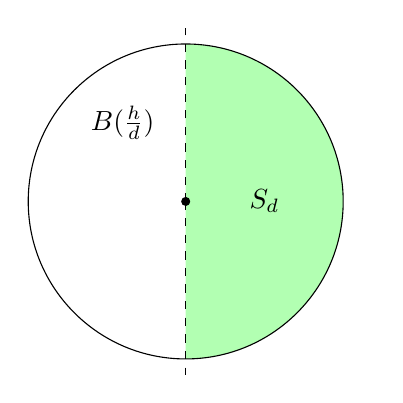
\begin{tikzpicture}
  \def\p{2}
  \def\D{1.2*\p}
  \def\th{90}

  \node[] at (0.95*\D,0) {$\Kc$};

  \fill [green!30] (0,0) --  (\th:\p) arc(\th:-\th:\p) -- cycle;

  \draw[dashed]
  (0,0) node[left] {$\xh$} coordinate (x) -- (0,1.1*\p) coordinate (top);
  \draw[dashed] (0,0) -- (0,-1.1*\p);

  \draw[] (0,0) circle (\p);
  \node[] at (-0.4*\p,0.5*\p) {$B_{\xh}(\frac{h}{d\Lcw})$};
  \draw[fill] (0,0) circle (.05);
  \node[] at (0.5*\p,0) {$S_d$};
\end{tikzpicture}
\hspace{10pt}
\raisebox{60pt}{$\geq$}
\hspace{10pt}
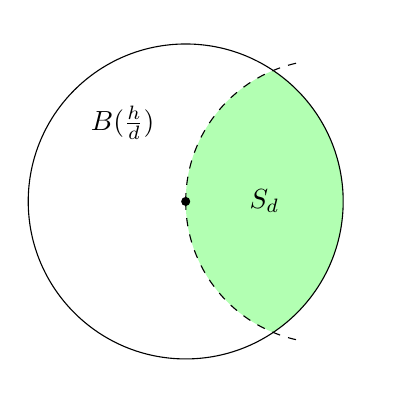
\begin{tikzpicture}
  \def\p{2}
  \def\D{1.2*\p}
  \def\r{1.8}

  \begin{scope}
    \clip(0,0) circle (\p);
    \fill[green!30](\r,0) circle (\r);
  \end{scope}

  \draw[dashed](0,0) arc(180:100:\r);
  \draw[dashed](0,0) arc(180:260:\r);

  \node[] at (0.95*\D,0) {$\Kc$};

  \node[] at (-0.25,0) {$\xh$};

  \draw[opacity=0] (0,0) -- (0,1.1*\p);
  \draw[opacity=0] (0,0) -- (0,-1.1*\p);

  \draw[] (0,0) circle (\p);
  \node[] at (-0.4*\p,0.5*\p) {$B_{\xh}(\frac{h}{d\Lcw})$};
  \draw[fill] (0,0) circle (.05);
  \node[] at (0.5*\p,0) {$S_d$};
\end{tikzpicture}
\hspace{10pt}
\raisebox{60pt}{$\geq$}
\hspace{10pt}
\begin{tikzpicture}
  \def\p{2}
  \def\D{1.2*\p}
  \def\th{45}

  \node[] at (0.95*\D,0) {$\Kc$};

  \fill [green!30] (0,0) --  (\th:\p) arc(\th:-\th:\p) -- cycle;

  \draw[dashed] 
  (0,0) node[left] {$\xh$} coordinate (x) -- ($({1.1*\p*cos(\th)},{1.1*\p*sin(\th)})$);
  \draw[dashed] (0,0) -- ($({1.1*\p*cos(\th)},-{1.1*\p*sin(\th)})$);

  \draw[opacity=0] (0,0) -- (0,1.1*\p);
  \draw[opacity=0] (0,0) -- (0,-1.1*\p);

  \draw[] (0,0) circle (\p);
  \node[] at (-0.4*\p,0.5*\p) {$B_{\xh}(\frac{h}{d\Lcw})$};
  \draw[fill] (0,0) circle (.05);
  \node[] at (0.6*\p,0) {$S_d$};
\end{tikzpicture}
\caption{\label{fig:apx:Kgeo} The intersection $\Kc\medcap 
B_{\xh}\!\left(\frac{h}{d\Lcw}\right)$ in green, for possible convex geometrical features on the 
boundary of $\Kc$ where the center $\xh$ can lie.}
\end{figure}

And so, there must exist at least one minimizing boundary location satisfying
$$
\mubKc(S_d)^\star \ := \ 
\min_{x\in\partial\Kc}\mubKc(S_d) \ = \ 
%\ps_\Kc\,\mubKc\!\left(B_{\xh}\!\left(\frac{h}{d\Lcw}\right)\right) \ = \ 
\frac{\ps_\Kc}{\Vc}\left(\frac{h}{d\Lcw}\right)^n\frac{\pi^{\frac{n}{2}}}{\Gamma(\frac{n}{2}+1)}
$$
for some $0<\ps_\Kc<\frac{1}{2}$, since $\Vc>0$ and the boundary of $\Kc$ must contain convex 
curved surfaces and/or vertices.

The exact portion $\ps_\Kc$ of the ball 
contained within $\mubKc(S_d)^\star$ may not be practical to calculate for a given $\Kc$, but we
can always lower bound it in the following manner (based on methods in
\cite{lamperski2021projected} Proof of Lemma 16, Case 1).

Denote $c_\Kc$ as the centroid of $\Kc$ and let $r$ be the radius of the largest ball centered
at $c_\Kc$ contained within $\Kc$. Then define $\ell\geq r$ as the distance from the centroid to 
the closest minimizing boundary location $x^\star$, and align a coordinate system at
$c_\Kc$ such that $x^\star$ is located at position $\big[-\ell\ \ 0\ \cdots\ 0\big]^\top$. Then
$x\in\Kc$ satisfying
$$
-\ell \ \leq x_1 \ \leq \ 0 \qquad \text{ and } \qquad
\sqrt{\sum_{i=2}^{n}x_i^2\,} \ \leq \ r + \frac{r}{\ell\,}\,x_1
$$
defines a conic section which is entirely within $\Kc$. If we then define
$$
\vartheta := \arctan\left(\frac{r}{\ell\,}\right)
\qquad\text{and}\qquad
\dscr + \dscr\sin(\vartheta) = \frac{h}{d\Lcw} \ \ ,
$$
this allows a ball of radius $\dscr\sin(\vartheta)$ to be inscribed within the conic section at
location $\big[-\ell+\dscr\ \ 0\ \cdots\ 0\big]^\top$.

Using the above definitions, we have that this radius satisfies
$$
\dscr\sin(\vartheta) \ = \ \frac{\frac{h}{d\Lcw}}{1+\sin(\vartheta)}\sin(\vartheta) \ = \ 
\frac{\frac{h}{d\Lcw}}{1 + \frac{r}{\sqrt{r^2 + \ell^2}\,}}\,\frac{r}{\sqrt{r^2 + 
\ell^2}\,}
\ = \ \frac{r}{r+\sqrt{r^2+\ell^2}}\,\frac{h}{d\Lcw} \ =: \ \varrho_\Kc\,\frac{h}{d\Lcw}
$$
and since the centroid is within the interior of $\Kc$, the factor $\varrho$ must satisfy
$$
\frac{r}{r+\sqrt{r^2+\Dc^2}\,} \ < \ \varrho_\Kc \ < \ \frac{r}{r+\sqrt{r^2 + r^2}\,} = 
\frac{1}{1+\sqrt{2}} \ \ .
$$
Figure~\ref{fig:apx:centroidK} illustrates an example of this method in $n=2$, with the 
inscribed ball outlined in red.
\begin{figure}[H]
\centering
\begin{tikzpicture}
  \def\r{1.6}
  \def\p{2}
  \def\th{45}
  \def\thC{20}
  \def\c{4.5}
  \def\D{7}
  \def\Dh{1.7}
  \def\DD{8}

  \fill [green!30] (0,0) --  (\th:\p) arc(\th:-\th:\p) -- cycle;

  \draw[dashed] (0,0) node[left] {$x^\star$} coordinate (x) --
  ($({1.1*\p*cos(\th)},{1.1*\p*sin(\th)})$) -- (\D,\Dh); % -- (\DD,0);
  \draw[dashed] (0,0) --
  ($({1.1*\p*cos(\th)},-{1.1*\p*sin(\th)})$) -- (\D,-\Dh); % -- (\DD,0);
  \draw[dashed] (\D,\Dh) arc(90:-90:\Dh);

  \fill [red!20] (0,0) --  (\thC:\p) arc(\thC:-\thC:\p) -- cycle;

  \draw[dotted] (\c,0) circle (\r);

  \draw[] (0,0) circle (\p);
  \node[] at (-0.4*\p,0.5*\p) {$B_{x^\star}(\frac{h}{d\Lcw})$};
  \draw[fill] (0,0) circle (.05);
  \node[] at (1.4,1.0) {$S_d$};

  \draw[] (0,0) -- (\c,\r) -- node[right] {$r$} (\c,0) -- (\c,-\r);
  \draw[] (0,0) -- (\c,-\r);

  \draw[-] (0,0) -- node[below right] {$\ell$} (\c,0);

  \node[] at (0.8,0.15) {$\vartheta$};

  \draw[fill] (\c,0) circle (.05);
  \node[] at (\c+.3,-0.25) {$c_\Kc$};

  \node[] at (7.3,1.1) {$\Kc$};

  \draw [thick,red] ($({\p*sqrt(\r*\r +\c*\c)/(\r+sqrt(\r*\r
    +\c*\c))},0)$) circle ({\p * \r/(\r + sqrt(\r*\r
    +\c*\c))});
  \draw[fill] ($({\p*sqrt(\r*\r +\c*\c)/(\r+sqrt(\r*\r
    +\c*\c))},0)$) node[below] {$\dscr$} circle (.05);
\end{tikzpicture}
\caption{\label{fig:apx:centroidK} The largest ball which always lower bounds $S_d$, centered at 
$\dscr$ with radius $\dscr\sin(\vartheta)$.}
\end{figure}

Thus, as $\xh$ moves toward such a minimizing boundary point of $\Kc$, we get the lower bound
$$
\mubKc(S_d) \ \geq \ 
\mubKc(S_d)^\star
%= \ps_\Kc\,\mubKc\!\left(B_{\xh}\!\left(\frac{h}{d\Lcw}\right)\right)
\ \geq \ \ 
\frac{\varrho_\Kc^n}{\Vc}\left(\frac{h}{d\Lcw}\right)^{\!n}\frac{\pi^{\frac{n}{2}}}{\Gamma(\frac{n}{2}+1)}
\ =: \ \frac{\rho_{\Kc,n}}{\Vc}\left(\frac{h}{d\Lcw}\right)^{\!n}
\ \ .
$$
On the other hand, there may be $x\in\Kc$ more than $\frac{h}{d\Lcw}$ away from any $\xh$ where
it still holds that $|\fw(x)|\geq\frac{d-1}{d}h$. Thus,
$$
S_d \subseteq\Omega_{\frac{d-1}{d}h}
\quad\implies\quad
\mubKc(S_d) \ \leq \ \mubKc\left(\Omega_{\frac{d-1}{d}h}\right)
\ \leq \ 
\frac{d^2\epsbase^2}{(d-1)^2h^2}
\ \ .
$$
Combining these relations gives that
$$
\frac{\rho_{\Kc,n}}{\Vc}\,\left(\frac{h}{d\Lcw}\right)^n \ \leq \ \mubKc(S_d) \ \leq \ 
\frac{d^2\epsbase^2}{(d-1)^2h^2}
\qquad\implies\qquad
h\ \leq \ \frac{d}{(d-1)^{\frac{2}{n+2}}}\,
\left(\frac{\Vc\Lcw^n\epsbase^2}{\rho_{\Kc,n}}\right)^{\frac{1}{n+2}}
$$
must hold for any $d\geq1$. Then since
$$
\frac{\d}{\d d}\frac{d}{(d-1)^{\frac{2}{n+2}}} \ = \ 
\frac{n(d-1)-2}{(n+2)(d-1)^{\frac{n+4}{n+2}}} = 0
\quad\implies\quad
d \ = \ \frac{n+2}{n} \ \ ,
$$
we have the smallest upper bound on $h$ as
$$
h\ \leq \ \frac{\frac{n+2}{n}}{\frac{2}{n}^{\frac{1}{n+2}}}
\left(\frac{\Vc\Lcw^n\epsbase^2}{\rho_{\Kc,n}}\right)^{\frac{1}{n+2}}
\ \leq \ 2\,(\rho_{\Kc,n})^{\frac{-1}{n+2}}\left(\Vc\Lcw^n\epsbase^2\right)^{\frac{1}{n+2}}
\ \ .
$$
By definition, we have
$$
(\rho_{\Kc,n})^{\frac{-1}{n+2}} \ = \
\left(\varrho_\Kc^n\,\frac{\pi^{\frac{n}{2}}}{\Gamma(\frac{n}{2}+1)}\right)^{\!\frac{-1}{n+2}}
\ = \ 
\left(\frac{r}{r+\sqrt{r^2+\ell^2}}\right)^{\!\frac{-n}{n+2}}
\left(\frac{\pi^{\frac{n}{2}}}{\Gamma(\frac{n}{2}+1)}\right)^{\!\frac{-1}{n+2}}
$$
and since $\Kc\subseteq B_0(\rho)$ for sufficiently large $\rho$, then
$$
\Vc \ \leq \ \rho^n\frac{\pi^{\frac{n}{2}}}{\Gamma(\frac{n}{2}+1)} \ \ .
$$
Thus,
$$
(\rho_{\Kc,n})^{\frac{-1}{n+2}}\,\Vc^{\frac{1}{n+2}} \ \leq \ 
\left(\frac{r}{r+\sqrt{r^2+\Dc^2}}\right)^{\!\frac{-n}{n+2}}\,\Dc^{\frac{n}{n+2}} \ \ .
$$
\vphantom{a}\hfill$\blacksquare$
